Based on the requirements outlined in~\ref{subsec:generalization_requirements} we can define the interface of a \texttt{Generalizer}.
Note, that since Go is not a classic object oriented language, a traditional class-hierarchy is not present in the design.
What we do have in our toolkit are \textit{interfaces} and \textit{composition}.

We define the \texttt{Generalizer} interface with the following operations (refer to Figure~\ref{fig:generalization_package}):
\begin{enumerate}
    \setstretch{1.0}
    \item generalize a partition \textit{n} times
    \item get the maximum number of levels of generalization
\end{enumerate}
Remember, that a partition can either contain a single value, or a set of values, so it makes sense that the \texttt{Generalize} method takes and returns a \texttt{Partition}.
It is also essential to know the maximum levels of generalization in advance, otherwise we wouldn't be able to compute the scaled generalization cost when comparing two partitions.
There is a third convenience method on the interface which defines how to create a \texttt{Partition} from a raw value.
The actual implementation of this may vary in each type that implements the interface.

\vspace{\baselineskip}
\begin{figure}
    \centering
    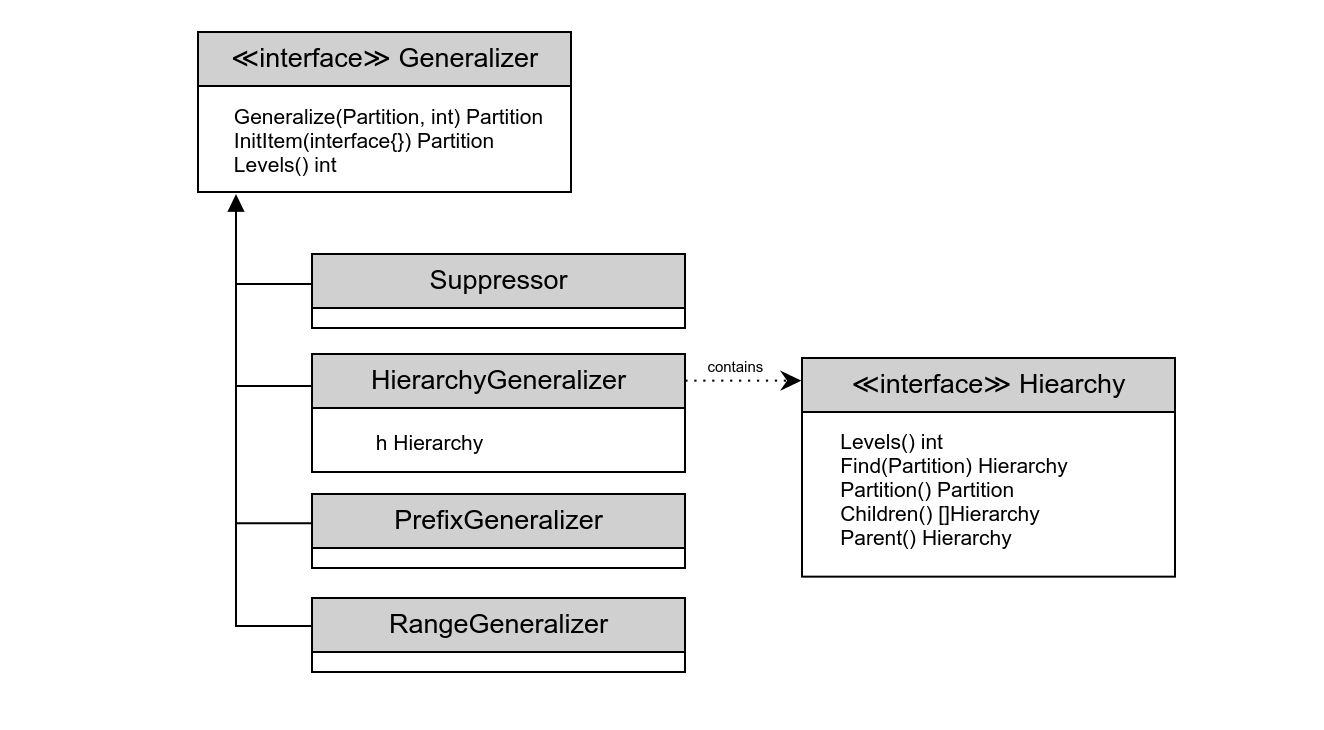
\includegraphics[width=\textwidth]{images/lib-generalizer.png}
    \caption{The generalization package}\label{fig:generalization_package}
\end{figure}

